\documentclass[sigconf, authorversion, nonacm]{acmart}
\settopmatter{printacmref=false}
\setcopyright{none}
\renewcommand\footnotetextcopyrightpermission[1]{}
\pagestyle{plain}

\usepackage{booktabs}

\begin{document}

\title{CollisionGuard: Pre-Execution Merge Conflict Forecasting and Scheduling for Concurrent Coding Agents}
\subtitle{Progress Report (Intermediate Draft)}

\author{Siddanagouda Patil}
\affiliation{\institution{}\country{}}
\author{Kanishq Upadhyay}
\affiliation{\institution{}\country{}}
\author{Mitansh Maheshwari}
\affiliation{\institution{}\country{}}

\begin{abstract}
Teams increasingly run several autonomous coding agents on the same repository at once. Their pull requests often collide at merge time, and the compute spent on the losing branch is wasted. We study \emph{pre-execution} conflict forecasting: given only an issue's text and repository history available before the task starts ($t_0$), can we predict which concurrent task pairs will fail to merge, and use that prediction to schedule them? CollisionGuard is a two-stage system. Stage~1 localizes each task's likely file footprint with hybrid BM25/dense retrieval, co-change mining and a LambdaMART re-ranker. Stage~2 turns the two footprint distributions into pairwise overlap features and feeds them to a monotonically constrained LightGBM classifier with out-of-fold isotonic calibration. A SimPy queue simulator then gates task pairs at a risk threshold $\tau$ and traces the trade-off between conflicts avoided and added delay. At the halfway point, the full pipeline is implemented and covered by 36 passing tests, together with ground-truth labeling through \texttt{git merge-tree}, a leakage-audit harness and a structural conflict taxonomy. We have \textbf{not yet run the pipeline on the real AIDev data}, so this draft contains no empirical claim about forecasting accuracy. We report what has been verified (software correctness and a scheduler sanity check on synthetic inputs) and lay out the evaluation plan for the remaining weeks.
\end{abstract}

\maketitle

\section{Introduction}
Agentic software engineering is moving from one assistant per developer to fleets of agents that each take an issue and open a pull request. When two agents edit overlapping files, or both touch a shared manifest such as \texttt{package.json}, at least one PR fails to merge cleanly. Rework is expensive: the agent run is already paid for, and the conflict is only discovered after execution. Existing practice is either to ignore the problem or to serialize all work on a repository, which discards the parallelism that motivates running many agents.

We ask whether conflicts can be forecast \emph{before} any agent runs, using only information available at $t_0$: the issue title and body, the repository file tree and its commit history up to $t_0$. A forecast of this kind would let a scheduler run likely-disjoint tasks in parallel and delay only the risky pairs. The problem has three properties that shape our design:
\begin{enumerate}
  \item \textbf{Strict pre-execution information.} Any feature derived from the diff, commit log or modified file list leaks the answer. We build leakage prevention and an explicit audit into the system.
  \item \textbf{Decisions depend on calibrated risk.} A scheduler needs a probability it can compare with a threshold, not just a ranking, so calibration is a first-class metric.
  \item \textbf{Class imbalance and asymmetric costs.} Conflicts are a minority outcome and a false hold costs differently from a missed conflict, so accuracy is uninformative.
\end{enumerate}

\paragraph{Contributions (planned).} (i) A two-stage footprint-then-conflict model with a monotonic guarantee in expected overlap; (ii) a leakage-audited, repository-isolated evaluation protocol; (iii) a discrete-event scheduling study that reports a Pareto frontier of conflicts avoided versus delay. This draft delivers the implementation of all three and the verification of their correctness; the empirical evaluation on real data is the main remaining work (Section~\ref{sec:plan}).

\section{Related Work}
\textbf{Textual merge conflicts.} Prior work characterizes how often and why merges conflict and predicts conflicts from branch-level signals available after development, such as changed-file overlap, line-level edits and developer activity. Our setting differs in that we predict before any code exists. \textbf{Early conflict awareness.} Tools such as speculative merging and workspace-awareness systems surface conflicts as soon as changes appear in a workspace, but still require edits to exist. \textbf{Bug and feature localization.} Information-retrieval-based localization ranks files for an issue using lexical and, more recently, embedding-based similarity, often combined with history signals such as co-change; we adopt this line for Stage~1. \textbf{Learning to rank and calibration.} LambdaMART optimizes NDCG for ranking; isotonic regression and expected calibration error are standard tools for probabilistic outputs. Monotonic constraints in gradient-boosted trees encode domain priors. \textbf{Scheduling with conflict prediction.} Conflict-aware scheduling is studied in databases and build systems; we apply it to agent PR queues. \emph{(Note: citations and a fuller literature survey are still to be added; none are verified yet, and we deliberately list no references rather than unchecked ones.)}

\section{Data}
\label{sec:data}
\paragraph{Source.} The target dataset is AIDev, a corpus of agent-authored pull requests with linked issues. The ingestion module streams PRs and issues through DuckDB under a memory limit to avoid out-of-memory failures on the full corpus.

\paragraph{Concurrent pairs and labels.} Two tasks form a candidate pair if they are in the same repository and their open--close intervals overlap in time. The pair label is obtained headlessly by replaying both PR heads with \texttt{git merge-tree}; exit codes are parsed into clean versus conflicting, and missing merge bases are handled explicitly. Conflicting pairs are further classified into a structural taxonomy (content, modify/delete, add/add).

\paragraph{Temporal validity.} Records are rejected unless the issue creation time precedes the PR open time ($T_{\text{issue}} \le T_{\text{open}}$), and co-change rules are mined only from commits before $t_0$.

\paragraph{Splits.} All evaluation uses repository-grouped $k$-fold splits so that no repository appears in both train and test, preventing cross-repository leakage of file names and history.

\paragraph{Status.} \textbf{The real AIDev data has not yet been ingested end to end.} The only data used so far are (a) small synthetic fixtures with scripted git repositories for unit tests and (b) a 36-task, 3-repository synthetic benchmark in \texttt{run\_pipeline.py}. Dataset statistics (number of repositories, PRs, concurrent pairs, conflict rate) will be reported here once the full run completes.

\section{Methods}
\subsection{Stage 1: File Footprint Localization}
For each task we retrieve candidate files from the repository tree at $t_0$ using BM25 and \texttt{all-MiniLM-L6-v2} dense embeddings, keeping a pool of up to 50 candidates. Each candidate gets a 15-dimensional feature vector, including path mentions in the issue, file churn, and lift of FP-Growth association rules mined from pre-$t_0$ commits. A LightGBM LambdaMART model re-ranks candidates (NDCG@10). Its output is read as $P(f \in F)$ for each file $f$. To avoid optimistic footprints in Stage~2 training, footprints for training tasks are generated out of fold.

\subsection{Stage 2: Pairwise Conflict Risk}
Given footprint distributions for tasks $A$ and $B$, we compute the expected overlap $E[|F_A\cap F_B|]=\sum_f p_A(f)\,p_B(f)$, the collision probability $P(|F_A\cap F_B|\ge 1)$, a build-manifest risk term for shared manifest files, and context features (issue-text similarity, recent repository churn, agent heterogeneity, temporal overlap). The nine features feed a LightGBM classifier with a monotone-increasing constraint on expected overlap, so that more predicted overlap can never lower predicted risk. Probabilities are calibrated by isotonic regression fit on out-of-fold predictions.

\subsection{Scheduling Simulation}
A SimPy discrete-event simulator replays chronological PR arrivals. When a new task's calibrated conflict probability with a running task is $\ge\tau$, it is held until the running task completes; otherwise it runs in parallel. Sweeping $\tau\in[0,1]$ yields a Pareto frontier of conflicts avoided against total queue delay, with a matched random-holding baseline planned for comparison.

\subsection{Baselines and Metrics}
Baselines: base rate; text cosine similarity of the two issues; a BM25 candidate-overlap heuristic; and an oracle that uses the \emph{true} modified-file footprints (an upper bound on what better localization could buy). Because conflicts are rare, we report PR-AUC as the primary ranking metric, with ROC-AUC, Brier score and expected calibration error (ECE) for probability quality. For Stage~1 we report Hit@$K$ and NDCG@10. For scheduling we report conflicts avoided (\%), conflicts missed, false-delay incidents and delay hours, since these map directly to cost.

\subsection{Leakage Audit and Interpretability}
The audit injects post-execution artifacts (diffs, commit logs, modified file names) into the inputs and measures metric inflation relative to the clean pipeline; a trustworthy pipeline should differ from the contaminated one only when the injected channel is actually usable. SHAP attributions for the Stage~2 model and a per-taxonomy breakdown of sub-metrics are implemented for analysis.

\section{Results}
\textbf{Important caveat: no result in this section measures real forecasting performance.} All numbers come from synthetic inputs and serve only to verify that the machinery runs and behaves sensibly.

\subsection{Software Verification}
The test suite (36 tests covering data validation, merge replay on scripted git repositories, localization, monotonic risk ordering, calibration, evaluation, simulation and an end-to-end integration test) passes in 33\,s on Python 3.12.

\subsection{Pipeline on the Synthetic Benchmark}
Running the cross-validated pipeline on the built-in 36-task synthetic benchmark produces degenerate metrics (Table~\ref{tab:synth}): the generated tasks each modify a single file in different positions, so \emph{no concurrent pair has a conflict label}. LightGBM reports zero positives in training, ROC-AUC is $0.5$ and PR-AUC is $0$ for every model including the oracle. This is a limitation of the toy generator, not evidence about the method, and it confirms that the real data run is required. We also note that the console banner in \texttt{run\_pipeline.py} says ``5-Fold'' while the default is 3 folds; this will be corrected.

\begin{table}[h]
  \caption{Synthetic 36-task benchmark (3 folds). All pairs are negatives, so ranking metrics are degenerate.}
  \label{tab:synth}
  \small
  \begin{tabular}{lcccc}
    \toprule
    Model & ROC & PR & ECE & Brier \\
    \midrule
    Base rate & 0.50 & 0.00 & 0.000 & 0.000 \\
    BM25 heuristic & 0.50 & 0.00 & 0.665 & 0.478 \\
    Text similarity & 0.50 & 0.00 & 0.673 & 0.454 \\
    CollisionGuard (Stage 2) & 0.50 & 0.00 & 0.000 & 0.000 \\
    CollisionGuard (calibrated) & 0.50 & 0.00 & 0.000 & 0.000 \\
    Oracle & 0.50 & 0.00 & 0.000 & 0.000 \\
    \bottomrule
  \end{tabular}
\end{table}

\subsection{Leakage Audit}
On the same synthetic data the audit reports zero difference between clean and contaminated runs (Stage~1 Hit@50 $1.00$ vs.\ $1.00$; Stage~2 PR-AUC $0.00$ vs.\ $0.00$). Since the metrics are saturated or degenerate, this passes trivially and does not yet validate isolation. The audit must be re-run on real data, where a non-zero inflation for deliberately contaminated inputs would show that the harness can detect leakage.

\subsection{Scheduler Sanity Check}
We swept $\tau$ on a synthetic workload of 50 tasks (Poisson arrivals, log-normal durations, 1--3 of 15 files each). Here the pairwise probabilities are \emph{drawn by hand from the true overlap} ($U[0.65,0.98]$ if files overlap, else $U[0.01,0.25]$), not predicted by our model, so the oracle-like separation is built in. Figure~\ref{fig:sim} shows the expected qualitative behaviour: very low $\tau$ holds many harmless pairs (3{,}410\,h of delay at $\tau=0$), a wide plateau ($\tau\in[0.25,0.65]$) avoids all 43 conflicts with 207\,h of delay and no false holds, and raising $\tau$ above $0.65$ trades missed conflicts for lower delay (e.g.\ 53\% avoided at $\tau=0.8$, 85\,h). The plateau reflects the artificial probability gap and should not be expected on real predictions. This experiment checks the simulator logic only.

\begin{figure}[h]
  \centering
  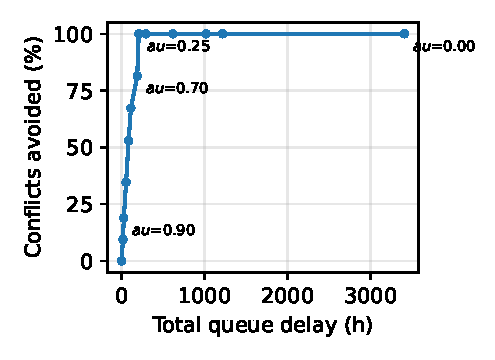
\includegraphics[width=0.95\columnwidth]{fig_sim_sanity.pdf}
  \caption{Scheduler sanity check on a synthetic workload with hand-set probabilities (not model output).}
  \label{fig:sim}
\end{figure}

\subsection{Figures to be Regenerated}
The repository's plotting script currently draws Hit@$K$ curves, PR curves and a reliability diagram from hard-coded or randomly generated values, not from pipeline output. These figures are \textbf{not} used in this report and must be rewritten to read real results before the final submission.

\section{Discussion}
The engineering of the pipeline is largely complete, but the central empirical question remains open: how well can pre-execution signals predict merge conflicts? Several risks are visible already. (1) Conflict rates in real agent PR data may be very low, making PR-AUC noisy and the Pareto frontier coarse. (2) Stage~1 errors propagate: if the true file is not in the top-50 pool, Stage~2 cannot see the overlap, and the oracle baseline will quantify this gap. (3) Some conflicts arise from files nobody would predict from text (generated files, lockfiles); the manifest feature addresses part of this. (4) Several Stage~2 context features are currently set to constants in the runner (text similarity $0.2$, churn $10$, heterogeneity false), which must be replaced by real values. (5) The merge-tree labels capture textual conflicts only, not semantic ones.

\section{Conclusion}
CollisionGuard's components are implemented and unit-tested, and the scheduler logic behaves as designed on synthetic input. Whether pre-execution forecasting is accurate enough to be useful is not yet established. Final conclusions are TBD pending the evaluation below.

\section{Remaining Work}
\label{sec:plan}
\begin{enumerate}
  \item \textbf{Real data run}: ingest AIDev, build concurrent pairs, label with \texttt{git merge-tree}, and report dataset statistics (Section~\ref{sec:data}).
  \item \textbf{Real evaluation}: repository-grouped CV for Stage~1 (Hit@$K$, NDCG@10) and Stage~2 (PR-AUC, ROC-AUC, Brier, ECE) with confidence intervals across folds, against all four baselines.
  \item \textbf{Ablations}: footprint source (BM25 / dense / hybrid / oracle), with and without the monotone constraint, with and without calibration.
  \item \textbf{Scheduling}: drive the simulator with the model's out-of-fold probabilities and real PR timestamps; add the matched random-holding baseline.
  \item \textbf{Leakage audit} on real data with a positive control.
  \item \textbf{Figures}: rewrite the plotting script to consume real outputs; remove hard-coded curves.
  \item \textbf{Literature}: complete the related-work survey and bibliography.
\end{enumerate}

\end{document}
